\documentclass[12pt]{article}
\usepackage{amsmath}
\usepackage{tikz}
\begin{document}
\title{Statistics 12, Homework 5}
\date{February 24th, 2019}
\author{Michael Wu\\UID: 404751542}
\maketitle

\section*{Chapter 14, Problem 2}

Let \(A\) be ``likes to cook'' and \(B\) be ``likes to shop''. Then we have the following.
\[P(A)\cup P(B) = P(A) + P(B) - P(A\cap B)=0.45 + 0.59 - 0.23=0.81\]

\section*{Chapter 14, Problem 4}

\[\frac{38}{38+22}\approx0.633\]

\section*{Chapter 14, Problem 6}

\[0.7\times0.9=0.63\]

\section*{Chapter 14, Problem 10}

\begin{center}
    \begin{tabular}{c|cc|c}
        & Bank Online & Does Not Bank Online & Total\\
        \hline
        Younger than 50 & 0.25 & 0.15 & 0.4\\
        Not Younger than 50 & 0.05 & 0.55 & 0.6\\
        \hline
        Total & 0.3 & 0.7 & 1
    \end{tabular}
\end{center}
A table is better than a tree here because it requires less calculation to use. Instead of having
to multiply probabilities to arrive at the given percentages, the table presents the data
in the same way that it's given to us.

\section*{Chapter 14, Problem 12}

\begin{center}
    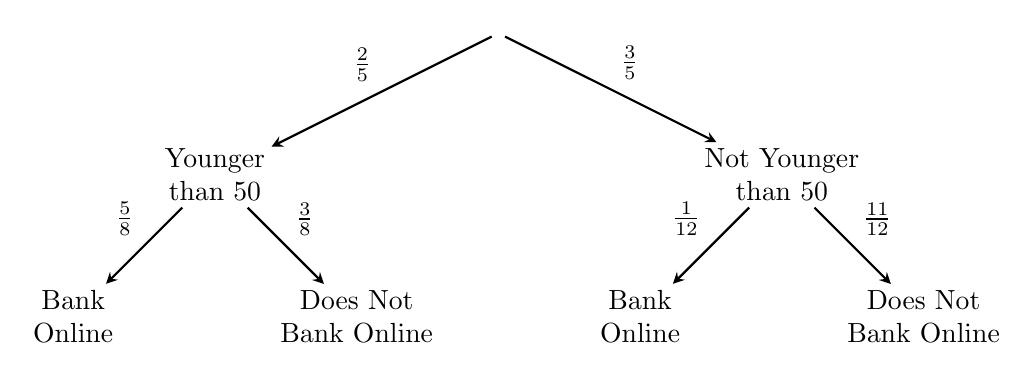
\begin{tikzpicture}[scale=0.9]
        \begin{scope}[auto, every node/.style={thick,rectangle,minimum size=0em,inner sep=2, align=center}]
            \node (Root) at (0,0) {};
            \node (Lt50) at (-4,-2) {Younger\\than 50};
            \node (Gt50) at (4,-2) {Not Younger\\than 50};
            \node (Online1) at (-6,-4) {Bank\\Online};
            \node (NotOnline1) at (-2,-4) {Does Not\\Bank Online};
            \node (Online2) at (2,-4) {Bank\\Online};
            \node (NotOnline2) at (6,-4) {Does Not\\Bank Online};
        \end{scope}
        \begin{scope}[auto, every node/.style={minimum size=0em}, every path/.style={thick, ->, >=stealth}]
            \path (Root) edge [above left] node {\(\frac{2}{5}\)} (Lt50);
            \path (Root) edge [above right] node {\(\frac{3}{5}\)}(Gt50);
            \path (Lt50) edge [above left] node {\(\frac{5}{8}\)} (Online1);
            \path (Lt50) edge [above right] node {\(\frac{3}{8}\)}(NotOnline1);
            \path (Gt50) edge [above left] node {\(\frac{1}{12}\)}(Online2);
            \path (Gt50) edge [above right] node {\(\frac{11}{12}\)}(NotOnline2);
        \end{scope}
    \end{tikzpicture}
\end{center}
A tree is better than a table in this case because we are given conditional probabilities. So it is easier
to express the probabilities in a way that matches the given data using a tree. The joint probabilities are
found by multiplying the conditional probabilities as you travel down a path in the tree.

\section*{Chapter 14, Problem 14}

\[\frac{\frac{2}{5}\times\frac{5}{8}}{\frac{2}{5}\times\frac{5}{8}+\frac{3}{5}\times\frac{1}{12}}\approx0.8333\]

\section*{Chapter 15, Problem 6}

I assume the mean score and standard deviation that is given applies to a single hole, and his total score is the
sum of the scores on each of the eighteen holes. His mean total score will then be
\[18\times85=1530\]
and the standard deviation of his total score will be
\[\sqrt{18\times11^2}\approx 46.669\]

\section*{Chapter 15, Problem 8}

This is the probability that a bottle of ketchup will have a z-score less than \(-2\). Using a calculator, I obtain
a probability of \(0.0228\).

\section*{Chapter 15, Problem 12}

\paragraph{a)}

The probability of winning \$100 is \(\frac{1}{6}\). The probability of winning \$50 is \(\frac{5}{36}\). The probability of
losing is \(\frac{25}{36}\).

\paragraph{b)}

I assume that I do not lose any money when I lose. Then the expected value of playing the game is the following.
\[100\times\frac{1}{6}+50\times\frac{5}{36}+0\times\frac{25}{36}\approx23.61\]

\paragraph{c)}

I would be willing to play this game since I would expect to win \$23.61 on average.

\section*{Chapter 16, Problem 4}

\[\binom{15}{2}0.08^2\times0.92^{13}\approx0.2273\]

\section*{Chapter 16, Problem 6}

\[\sum_{n=23}^{200}\binom{200}{n}0.08^n\times0.92^{200-n}\approx0.05066\]

\section*{Chapter 16, Problem 28}

\paragraph{a)}

The expected value of the number of times the ball winds up in a green slot is \(2\) times.

\paragraph{b)}

The ball has a \(\frac{2}{38}\) chance of landing in a green slot on each spin. Thus the expected
value of the number of times the ball winds up in a green slot after 38 spins is the following.
\[38\times\frac{2}{38}=2\]

\end{document}